\documentclass{article}
\usepackage{tikz} 

\begin{document}
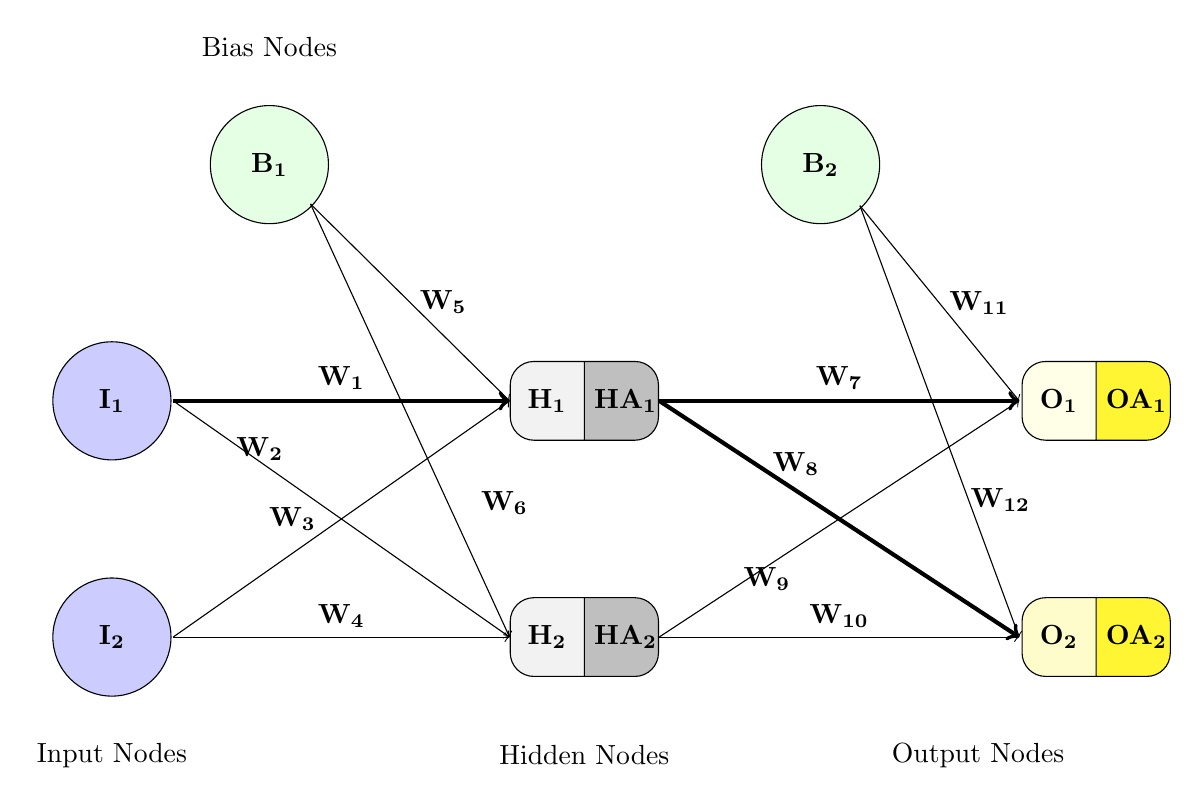
\begin{tikzpicture}
\usetikzlibrary {quotes}
\usetikzlibrary {shapes,positioning}
  \node[minimum size=1.5cm,fill=green!10!white,draw,circle]  at (0,0){ $\mathbf{B_1}$};
  \node[minimum size=1.5cm,fill=green!10!white,draw,circle]  at (7,0){ $\mathbf{B_2}$};
` \node  at (0,1.5) {Bias Nodes};
\node[minimum size=1.5cm,fill=blue!20!white,draw,circle] (i1) at (-2,-3){ $\mathbf{I_1}$};
\node[minimum size=1.5cm,fill=blue!20!white,draw,circle] (i2) at (-2,-6){ $\mathbf{I_2}$};
\node[minimum height=1cm,,minimum width=4cm,rectangle split,rectangle split 
    horizontal, 
    rectangle split parts=2,text width=0.7cm,text centered,
    rectangle split part fill={black!5,black!25},
    rounded corners=0.3cm, draw]  at (4,-3) {$\mathbf{H_1}$ \nodepart{two} $\mathbf{HA_1}$ };
\node[minimum height=1cm,,minimum width=4cm,rectangle split,rectangle split 
    horizontal, 
    rectangle split parts=2,text width=0.7cm,text centered,
    rectangle split part fill={yellow!10,yellow!80},
    rounded corners=0.3cm, draw]  at (10.5,-3) {$\mathbf{O_1}$ \nodepart{two} $\mathbf{OA_1}$  };
\node[minimum height=1cm,,minimum width=4cm,rectangle split,rectangle split 
    horizontal, 
    rectangle split parts=2,text width=0.7cm,text centered,
    rectangle split part fill={black!5,black!25},
    rounded corners=0.3cm, draw]  at (4,-6) {$\mathbf{H_2}$ \nodepart{two} $\mathbf{HA_2}$ };
\node[minimum height=1cm,,minimum width=4cm,rectangle split,rectangle split 
    horizontal, 
    rectangle split parts=2,text width=0.7cm,text centered,
    rectangle split part fill={yellow!20,yellow!80},
    rounded corners=0.3cm,draw]  at (10.5,-6) {$\mathbf{O_2}$ \nodepart{two} $\mathbf{OA_2}$ };

\node  at (-2,-7.5) {Input Nodes};
\node  at (4,-7.5) {Hidden Nodes};
\node  at (9,-7.5) {Output Nodes};
\draw[->, line width=1.5pt] (-1.22222,-3) -> (3.05,-3) node[midway, above] {$\mathbf{W_1}$};
\draw[->] (-1.22222,-3) -> (3.05,-6) node[midway, above left=0.867] {$\mathbf{W_2}$};
\draw[->] (-1.22222,-6) -> (3.05,-3) node[midway, left = 0.2] {$\mathbf{W_3}$};
\draw[->] (-1.22222,-6) -> (3.05,-6) node[midway, above] {$\mathbf{W_4}$};
\draw[->] (0.522, -0.5) -- (3.05,-3) node[midway, right] {$\mathbf{W_5}$};
\draw[->] (0.522, -0.5) -- (3.05,-6) node[midway, below right=1.1] {$\mathbf{W_6}$};
\draw[->, line width=1.5pt] (4.95,-3) -- (9.522, -3) node[midway, above] {$\mathbf{W_7}$};
\draw[->, line width=1.5pt] (4.95,-3) -> (9.522,-6) node[midway, below right = -1.4] {$\mathbf{W_8}$};
\draw[->] (4.95,-6) -- (9.522, -3) node[midway, below left=0.7 ] {$\mathbf{W_9}$};
\draw[->] (4.95,-6) -- (9.522,-6) node[midway, above] {$\mathbf{W_{10}}$};
\draw[->] (7.5,-0.522) -- (9.522, -3) node[midway, right] {$\mathbf{W_{11}}$};
\draw[->] (7.5,-0.522) -- (9.522,-6) node[midway, above left =-1.8] {$\mathbf{W_{12}}$};
\end{tikzpicture}
\end{document}